% Options for packages loaded elsewhere
\PassOptionsToPackage{unicode}{hyperref}
\PassOptionsToPackage{hyphens}{url}
%
\documentclass[
]{article}
\usepackage{amsmath,amssymb}
\usepackage{iftex}
\ifPDFTeX
  \usepackage[T1]{fontenc}
  \usepackage[utf8]{inputenc}
  \usepackage{textcomp} % provide euro and other symbols
\else % if luatex or xetex
  \usepackage{unicode-math} % this also loads fontspec
  \defaultfontfeatures{Scale=MatchLowercase}
  \defaultfontfeatures[\rmfamily]{Ligatures=TeX,Scale=1}
\fi
\usepackage{lmodern}
\ifPDFTeX\else
  % xetex/luatex font selection
\fi
% Use upquote if available, for straight quotes in verbatim environments
\IfFileExists{upquote.sty}{\usepackage{upquote}}{}
\IfFileExists{microtype.sty}{% use microtype if available
  \usepackage[]{microtype}
  \UseMicrotypeSet[protrusion]{basicmath} % disable protrusion for tt fonts
}{}
\makeatletter
\@ifundefined{KOMAClassName}{% if non-KOMA class
  \IfFileExists{parskip.sty}{%
    \usepackage{parskip}
  }{% else
    \setlength{\parindent}{0pt}
    \setlength{\parskip}{6pt plus 2pt minus 1pt}}
}{% if KOMA class
  \KOMAoptions{parskip=half}}
\makeatother
\usepackage{xcolor}
\usepackage[margin=1in]{geometry}
\usepackage{color}
\usepackage{fancyvrb}
\newcommand{\VerbBar}{|}
\newcommand{\VERB}{\Verb[commandchars=\\\{\}]}
\DefineVerbatimEnvironment{Highlighting}{Verbatim}{commandchars=\\\{\}}
% Add ',fontsize=\small' for more characters per line
\usepackage{framed}
\definecolor{shadecolor}{RGB}{248,248,248}
\newenvironment{Shaded}{\begin{snugshade}}{\end{snugshade}}
\newcommand{\AlertTok}[1]{\textcolor[rgb]{0.94,0.16,0.16}{#1}}
\newcommand{\AnnotationTok}[1]{\textcolor[rgb]{0.56,0.35,0.01}{\textbf{\textit{#1}}}}
\newcommand{\AttributeTok}[1]{\textcolor[rgb]{0.13,0.29,0.53}{#1}}
\newcommand{\BaseNTok}[1]{\textcolor[rgb]{0.00,0.00,0.81}{#1}}
\newcommand{\BuiltInTok}[1]{#1}
\newcommand{\CharTok}[1]{\textcolor[rgb]{0.31,0.60,0.02}{#1}}
\newcommand{\CommentTok}[1]{\textcolor[rgb]{0.56,0.35,0.01}{\textit{#1}}}
\newcommand{\CommentVarTok}[1]{\textcolor[rgb]{0.56,0.35,0.01}{\textbf{\textit{#1}}}}
\newcommand{\ConstantTok}[1]{\textcolor[rgb]{0.56,0.35,0.01}{#1}}
\newcommand{\ControlFlowTok}[1]{\textcolor[rgb]{0.13,0.29,0.53}{\textbf{#1}}}
\newcommand{\DataTypeTok}[1]{\textcolor[rgb]{0.13,0.29,0.53}{#1}}
\newcommand{\DecValTok}[1]{\textcolor[rgb]{0.00,0.00,0.81}{#1}}
\newcommand{\DocumentationTok}[1]{\textcolor[rgb]{0.56,0.35,0.01}{\textbf{\textit{#1}}}}
\newcommand{\ErrorTok}[1]{\textcolor[rgb]{0.64,0.00,0.00}{\textbf{#1}}}
\newcommand{\ExtensionTok}[1]{#1}
\newcommand{\FloatTok}[1]{\textcolor[rgb]{0.00,0.00,0.81}{#1}}
\newcommand{\FunctionTok}[1]{\textcolor[rgb]{0.13,0.29,0.53}{\textbf{#1}}}
\newcommand{\ImportTok}[1]{#1}
\newcommand{\InformationTok}[1]{\textcolor[rgb]{0.56,0.35,0.01}{\textbf{\textit{#1}}}}
\newcommand{\KeywordTok}[1]{\textcolor[rgb]{0.13,0.29,0.53}{\textbf{#1}}}
\newcommand{\NormalTok}[1]{#1}
\newcommand{\OperatorTok}[1]{\textcolor[rgb]{0.81,0.36,0.00}{\textbf{#1}}}
\newcommand{\OtherTok}[1]{\textcolor[rgb]{0.56,0.35,0.01}{#1}}
\newcommand{\PreprocessorTok}[1]{\textcolor[rgb]{0.56,0.35,0.01}{\textit{#1}}}
\newcommand{\RegionMarkerTok}[1]{#1}
\newcommand{\SpecialCharTok}[1]{\textcolor[rgb]{0.81,0.36,0.00}{\textbf{#1}}}
\newcommand{\SpecialStringTok}[1]{\textcolor[rgb]{0.31,0.60,0.02}{#1}}
\newcommand{\StringTok}[1]{\textcolor[rgb]{0.31,0.60,0.02}{#1}}
\newcommand{\VariableTok}[1]{\textcolor[rgb]{0.00,0.00,0.00}{#1}}
\newcommand{\VerbatimStringTok}[1]{\textcolor[rgb]{0.31,0.60,0.02}{#1}}
\newcommand{\WarningTok}[1]{\textcolor[rgb]{0.56,0.35,0.01}{\textbf{\textit{#1}}}}
\usepackage{longtable,booktabs,array}
\usepackage{calc} % for calculating minipage widths
% Correct order of tables after \paragraph or \subparagraph
\usepackage{etoolbox}
\makeatletter
\patchcmd\longtable{\par}{\if@noskipsec\mbox{}\fi\par}{}{}
\makeatother
% Allow footnotes in longtable head/foot
\IfFileExists{footnotehyper.sty}{\usepackage{footnotehyper}}{\usepackage{footnote}}
\makesavenoteenv{longtable}
\usepackage{graphicx}
\makeatletter
\newsavebox\pandoc@box
\newcommand*\pandocbounded[1]{% scales image to fit in text height/width
  \sbox\pandoc@box{#1}%
  \Gscale@div\@tempa{\textheight}{\dimexpr\ht\pandoc@box+\dp\pandoc@box\relax}%
  \Gscale@div\@tempb{\linewidth}{\wd\pandoc@box}%
  \ifdim\@tempb\p@<\@tempa\p@\let\@tempa\@tempb\fi% select the smaller of both
  \ifdim\@tempa\p@<\p@\scalebox{\@tempa}{\usebox\pandoc@box}%
  \else\usebox{\pandoc@box}%
  \fi%
}
% Set default figure placement to htbp
\def\fps@figure{htbp}
\makeatother
\setlength{\emergencystretch}{3em} % prevent overfull lines
\providecommand{\tightlist}{%
  \setlength{\itemsep}{0pt}\setlength{\parskip}{0pt}}
\setcounter{secnumdepth}{-\maxdimen} % remove section numbering
\usepackage{bookmark}
\IfFileExists{xurl.sty}{\usepackage{xurl}}{} % add URL line breaks if available
\urlstyle{same}
\hypersetup{
  pdftitle={Tarea-Script.R},
  pdfauthor={Usuario},
  hidelinks,
  pdfcreator={LaTeX via pandoc}}

\title{Tarea-Script.R}
\author{Usuario}
\date{2025-09-22}

\begin{document}
\maketitle

\begin{Shaded}
\begin{Highlighting}[]
\CommentTok{\# Andrea Michelle Luna Vasconcelos 1950889}
\CommentTok{\# Tarea{-} Ejercicio ANOVA 22/09/2025}

\CommentTok{\# Comparación de concentraciones de estroncio en cuerpos de agua}

\CommentTok{\# Descripción{-}Datos a trabajar {-}{-}{-}{-}{-}{-}{-}{-}{-}{-}{-}{-}{-}{-}{-}{-}{-}{-}{-}{-}{-}{-}{-}{-}{-}{-}{-}{-}{-}{-}{-}{-}{-}{-}{-}{-}{-}{-}{-}{-}{-}{-}{-}{-}}

\NormalTok{estroncio }\OtherTok{\textless{}{-}} \FunctionTok{read.csv}\NormalTok{(}\StringTok{"C:/Repositorio GitHub/Posgrado\_Estadistica\_2025/Tarea 22\_09/Estroncio mg\_ml.csv"}\NormalTok{)}
\FunctionTok{View}\NormalTok{(estroncio)}

\FunctionTok{library}\NormalTok{(knitr)}
\FunctionTok{kable}\NormalTok{(}\FunctionTok{head}\NormalTok{(estroncio), }\AttributeTok{caption =} \StringTok{"Concentración de estroncio (mg/ml)}
\StringTok{      en cinco cuerpos de agua (n=6)"}\NormalTok{)}
\end{Highlighting}
\end{Shaded}

\begin{longtable}[]{@{}
  >{\raggedleft\arraybackslash}p{(\linewidth - 10\tabcolsep) * \real{0.1067}}
  >{\raggedleft\arraybackslash}p{(\linewidth - 10\tabcolsep) * \real{0.2000}}
  >{\raggedleft\arraybackslash}p{(\linewidth - 10\tabcolsep) * \real{0.1600}}
  >{\raggedleft\arraybackslash}p{(\linewidth - 10\tabcolsep) * \real{0.1867}}
  >{\raggedleft\arraybackslash}p{(\linewidth - 10\tabcolsep) * \real{0.2000}}
  >{\raggedleft\arraybackslash}p{(\linewidth - 10\tabcolsep) * \real{0.1467}}@{}}
\caption{Concentración de estroncio (mg/ml) en cinco cuerpos de agua
(n=6)}\tabularnewline
\toprule\noalign{}
\begin{minipage}[b]{\linewidth}\raggedleft
Muestra
\end{minipage} & \begin{minipage}[b]{\linewidth}\raggedleft
Grayson.s.Pond
\end{minipage} & \begin{minipage}[b]{\linewidth}\raggedleft
Beaver.Lake
\end{minipage} & \begin{minipage}[b]{\linewidth}\raggedleft
Angler.s.Cove
\end{minipage} & \begin{minipage}[b]{\linewidth}\raggedleft
Appletree.Lake
\end{minipage} & \begin{minipage}[b]{\linewidth}\raggedleft
Rock.River
\end{minipage} \\
\midrule\noalign{}
\endfirsthead
\toprule\noalign{}
\begin{minipage}[b]{\linewidth}\raggedleft
Muestra
\end{minipage} & \begin{minipage}[b]{\linewidth}\raggedleft
Grayson.s.Pond
\end{minipage} & \begin{minipage}[b]{\linewidth}\raggedleft
Beaver.Lake
\end{minipage} & \begin{minipage}[b]{\linewidth}\raggedleft
Angler.s.Cove
\end{minipage} & \begin{minipage}[b]{\linewidth}\raggedleft
Appletree.Lake
\end{minipage} & \begin{minipage}[b]{\linewidth}\raggedleft
Rock.River
\end{minipage} \\
\midrule\noalign{}
\endhead
\bottomrule\noalign{}
\endlastfoot
1 & 28.2 & 39.6 & 46.3 & 41.0 & 56.3 \\
2 & 33.2 & 40.8 & 42.1 & 44.1 & 54.1 \\
3 & 36.4 & 37.9 & 43.5 & 46.4 & 59.4 \\
4 & 34.6 & 37.1 & 48.8 & 40.2 & 62.7 \\
5 & 29.1 & 43.6 & 43.7 & 38.6 & 60.0 \\
6 & 31.0 & 42.4 & 40.1 & 36.3 & 57.3 \\
\end{longtable}

\begin{Shaded}
\begin{Highlighting}[]
\FunctionTok{library}\NormalTok{(tidyverse)}
\end{Highlighting}
\end{Shaded}

\begin{verbatim}
## -- Attaching core tidyverse packages ------------------------ tidyverse 2.0.0 --
## v dplyr     1.1.4     v readr     2.1.5
## v forcats   1.0.0     v stringr   1.5.1
## v ggplot2   3.5.2     v tibble    3.3.0
## v lubridate 1.9.4     v tidyr     1.3.1
## v purrr     1.1.0     
## -- Conflicts ------------------------------------------ tidyverse_conflicts() --
## x dplyr::filter() masks stats::filter()
## x dplyr::lag()    masks stats::lag()
## i Use the conflicted package (<http://conflicted.r-lib.org/>) to force all conflicts to become errors
\end{verbatim}

\begin{Shaded}
\begin{Highlighting}[]
\NormalTok{estroncio\_long }\OtherTok{\textless{}{-}}\NormalTok{ estroncio }\SpecialCharTok{\%\textgreater{}\%}
  \FunctionTok{pivot\_longer}\NormalTok{(}\AttributeTok{cols=} \SpecialCharTok{{-}}\NormalTok{Muestra,}
               \AttributeTok{names\_to =} \StringTok{"Cuerpo\_agua"}\NormalTok{,}
               \AttributeTok{values\_to =} \StringTok{"Concentracion"}\NormalTok{)}
\FunctionTok{view}\NormalTok{(estroncio\_long)}

\CommentTok{\# Convertir en factor el cuerpo de agua}

\NormalTok{estroncio\_long}\SpecialCharTok{$}\NormalTok{Cuerpo\_agua }\OtherTok{\textless{}{-}} \FunctionTok{as.factor}\NormalTok{(estroncio\_long}\SpecialCharTok{$}\NormalTok{Cuerpo\_agua)}

\FunctionTok{kable}\NormalTok{(}\FunctionTok{head}\NormalTok{(estroncio\_long), }\AttributeTok{caption =} \StringTok{"Datos reorganizados de concentraciones}
\StringTok{      de estroncio (mg/ml) en cinco cuerpos de agua como factor"}\NormalTok{)}
\end{Highlighting}
\end{Shaded}

\begin{longtable}[]{@{}rlr@{}}
\caption{Datos reorganizados de concentraciones de estroncio (mg/ml) en
cinco cuerpos de agua como factor}\tabularnewline
\toprule\noalign{}
Muestra & Cuerpo\_agua & Concentracion \\
\midrule\noalign{}
\endfirsthead
\toprule\noalign{}
Muestra & Cuerpo\_agua & Concentracion \\
\midrule\noalign{}
\endhead
\bottomrule\noalign{}
\endlastfoot
1 & Grayson.s.Pond & 28.2 \\
1 & Beaver.Lake & 39.6 \\
1 & Angler.s.Cove & 46.3 \\
1 & Appletree.Lake & 41.0 \\
1 & Rock.River & 56.3 \\
2 & Grayson.s.Pond & 33.2 \\
\end{longtable}

\begin{Shaded}
\begin{Highlighting}[]
\FunctionTok{summary}\NormalTok{(estroncio\_long)}
\end{Highlighting}
\end{Shaded}

\begin{verbatim}
##     Muestra            Cuerpo_agua Concentracion  
##  Min.   :1.0   Angler.s.Cove :6    Min.   :28.20  
##  1st Qu.:2.0   Appletree.Lake:6    1st Qu.:37.30  
##  Median :3.5   Beaver.Lake   :6    Median :41.55  
##  Mean   :3.5   Grayson.s.Pond:6    Mean   :43.16  
##  3rd Qu.:5.0   Rock.River    :6    3rd Qu.:46.38  
##  Max.   :6.0                       Max.   :62.70
\end{verbatim}

\begin{Shaded}
\begin{Highlighting}[]
\FunctionTok{tapply}\NormalTok{(estroncio\_long}\SpecialCharTok{$}\NormalTok{Concentracion, estroncio\_long}\SpecialCharTok{$}\NormalTok{Cuerpo\_agua, mean)}
\end{Highlighting}
\end{Shaded}

\begin{verbatim}
##  Angler.s.Cove Appletree.Lake    Beaver.Lake Grayson.s.Pond     Rock.River 
##       44.08333       41.10000       40.23333       32.08333       58.30000
\end{verbatim}

\begin{Shaded}
\begin{Highlighting}[]
\CommentTok{\# Angler.s.Cove   Appletree.Lake    Beaver.Lake  Grayson.s.Pond   Rock.River }
\CommentTok{\#  44.08333        41.10000         40.23333       32.08333       58.30000}

  

\CommentTok{\# Preguntas {-}{-}{-}{-}{-}{-}{-}{-}{-}{-}{-}{-}{-}{-}{-}{-}{-}{-}{-}{-}{-}{-}{-}{-}{-}{-}{-}{-}{-}{-}{-}{-}{-}{-}{-}{-}{-}{-}{-}{-}{-}{-}{-}{-}{-}{-}{-}{-}{-}{-}{-}{-}{-}{-}{-}{-}{-}{-}{-}{-}{-}{-}{-}}

\CommentTok{\# Hipótesis del ANOVA {-}{-}{-}{-}{-}{-}{-}{-}{-}{-}{-}{-}{-}{-}{-}{-}{-}{-}{-}{-}{-}{-}{-}{-}{-}{-}{-}{-}{-}{-}{-}{-}{-}{-}{-}{-}{-}{-}{-}{-}{-}{-}{-}{-}{-}{-}{-}{-}{-}{-}{-}{-}{-}}

\CommentTok{\# H0 = La media de concentración de estroncio en todos los cuerpos de agua son }
\CommentTok{\# iguales.}
\CommentTok{\# H1 = Al menos una media de concentración de estroncio es diferente al resto}
\CommentTok{\# de las medias de los cuerpos de agua.}

\CommentTok{\# Cálculo del ANOVA {-}{-}{-}{-}{-}{-}{-}{-}{-}{-}{-}{-}{-}{-}{-}{-}{-}{-}{-}{-}{-}{-}{-}{-}{-}{-}{-}{-}{-}{-}{-}{-}{-}{-}{-}{-}{-}{-}{-}{-}{-}{-}{-}{-}{-}{-}{-}{-}{-}{-}{-}{-}{-}{-}{-}}

\FunctionTok{bartlett.test}\NormalTok{(estroncio\_long}\SpecialCharTok{$}\NormalTok{Concentracion }\SpecialCharTok{\textasciitilde{}}\NormalTok{ estroncio\_long}\SpecialCharTok{$}\NormalTok{Cuerpo\_agua)}
\end{Highlighting}
\end{Shaded}

\begin{verbatim}
## 
##  Bartlett test of homogeneity of variances
## 
## data:  estroncio_long$Concentracion by estroncio_long$Cuerpo_agua
## Bartlett's K-squared = 0.63895, df = 4, p-value = 0.9586
\end{verbatim}

\begin{Shaded}
\begin{Highlighting}[]
  \CommentTok{\# p vale = 0.9586, son homogeneas}
 
\NormalTok{estroncio\_long.aov }\OtherTok{\textless{}{-}} \FunctionTok{aov}\NormalTok{(estroncio\_long}\SpecialCharTok{$}\NormalTok{Concentracion }\SpecialCharTok{\textasciitilde{}}\NormalTok{ estroncio\_long}\SpecialCharTok{$}\NormalTok{Cuerpo\_agua) }
\FunctionTok{summary}\NormalTok{(estroncio\_long.aov)}
\end{Highlighting}
\end{Shaded}

\begin{verbatim}
##                            Df Sum Sq Mean Sq F value   Pr(>F)    
## estroncio_long$Cuerpo_agua  4 2193.4   548.4   56.16 3.95e-12 ***
## Residuals                  25  244.1     9.8                     
## ---
## Signif. codes:  0 '***' 0.001 '**' 0.01 '*' 0.05 '.' 0.1 ' ' 1
\end{verbatim}

\begin{Shaded}
\begin{Highlighting}[]
\FunctionTok{library}\NormalTok{(broom)}
\FunctionTok{library}\NormalTok{(knitr)  }

\NormalTok{anova }\OtherTok{\textless{}{-}} \FunctionTok{tidy}\NormalTok{(estroncio\_long.aov)}
\FunctionTok{kable}\NormalTok{(anova, }\AttributeTok{caption =} \StringTok{"Resultados de análisis de varianza (ANOVA de una vía)"}\NormalTok{)  }
\end{Highlighting}
\end{Shaded}

\begin{longtable}[]{@{}
  >{\raggedright\arraybackslash}p{(\linewidth - 10\tabcolsep) * \real{0.4091}}
  >{\raggedleft\arraybackslash}p{(\linewidth - 10\tabcolsep) * \real{0.0455}}
  >{\raggedleft\arraybackslash}p{(\linewidth - 10\tabcolsep) * \real{0.1364}}
  >{\raggedleft\arraybackslash}p{(\linewidth - 10\tabcolsep) * \real{0.1364}}
  >{\raggedleft\arraybackslash}p{(\linewidth - 10\tabcolsep) * \real{0.1515}}
  >{\raggedleft\arraybackslash}p{(\linewidth - 10\tabcolsep) * \real{0.1212}}@{}}
\caption{Resultados de análisis de varianza (ANOVA de una
vía)}\tabularnewline
\toprule\noalign{}
\begin{minipage}[b]{\linewidth}\raggedright
term
\end{minipage} & \begin{minipage}[b]{\linewidth}\raggedleft
df
\end{minipage} & \begin{minipage}[b]{\linewidth}\raggedleft
sumsq
\end{minipage} & \begin{minipage}[b]{\linewidth}\raggedleft
meansq
\end{minipage} & \begin{minipage}[b]{\linewidth}\raggedleft
statistic
\end{minipage} & \begin{minipage}[b]{\linewidth}\raggedleft
p.value
\end{minipage} \\
\midrule\noalign{}
\endfirsthead
\toprule\noalign{}
\begin{minipage}[b]{\linewidth}\raggedright
term
\end{minipage} & \begin{minipage}[b]{\linewidth}\raggedleft
df
\end{minipage} & \begin{minipage}[b]{\linewidth}\raggedleft
sumsq
\end{minipage} & \begin{minipage}[b]{\linewidth}\raggedleft
meansq
\end{minipage} & \begin{minipage}[b]{\linewidth}\raggedleft
statistic
\end{minipage} & \begin{minipage}[b]{\linewidth}\raggedleft
p.value
\end{minipage} \\
\midrule\noalign{}
\endhead
\bottomrule\noalign{}
\endlastfoot
estroncio\_long\$Cuerpo\_agua & 4 & 2193.442 & 548.3605 & 56.15456 &
0 \\
Residuals & 25 & 244.130 & 9.7652 & NA & NA \\
\end{longtable}

\begin{Shaded}
\begin{Highlighting}[]
\CommentTok{\# H0 = (medias iguales) = se rechaza}
\CommentTok{\# H1 = (al menos una media distinta) = se acepta}

\CommentTok{\# Prueba LSD {-}{-}{-}{-}{-}{-}{-}{-}{-}{-}{-}{-}{-}{-}{-}{-}{-}{-}{-}{-}{-}{-}{-}{-}{-}{-}{-}{-}{-}{-}{-}{-}{-}{-}{-}{-}{-}{-}{-}{-}{-}{-}{-}{-}{-}{-}{-}{-}{-}{-}{-}{-}{-}{-}{-}{-}{-}{-}{-}{-}{-}{-}}

\FunctionTok{library}\NormalTok{(ggplot2)}

\FunctionTok{ggplot}\NormalTok{(estroncio\_long, }\FunctionTok{aes}\NormalTok{(}\AttributeTok{x =}\NormalTok{ Cuerpo\_agua, }\AttributeTok{y =}\NormalTok{ Concentracion, }\AttributeTok{fill =}\NormalTok{ Cuerpo\_agua)) }\SpecialCharTok{+}
  \FunctionTok{geom\_violin}\NormalTok{(}\AttributeTok{trim =} \ConstantTok{FALSE}\NormalTok{, }\AttributeTok{alpha =} \FloatTok{0.5}\NormalTok{) }\SpecialCharTok{+}
  \FunctionTok{geom\_boxplot}\NormalTok{(}\AttributeTok{width =} \FloatTok{0.1}\NormalTok{, }\AttributeTok{fill =} \StringTok{"white"}\NormalTok{, }\AttributeTok{outlier.shape =} \ConstantTok{NA}\NormalTok{) }\SpecialCharTok{+}
  \FunctionTok{geom\_jitter}\NormalTok{(}\AttributeTok{width =} \FloatTok{0.1}\NormalTok{, }\AttributeTok{size =} \DecValTok{2}\NormalTok{, }\AttributeTok{alpha =} \FloatTok{0.7}\NormalTok{) }\SpecialCharTok{+}
  \FunctionTok{labs}\NormalTok{(}
    \AttributeTok{title =} \StringTok{"Concentraciones de estroncio en cuerpos de agua"}\NormalTok{,}
    \AttributeTok{x =} \StringTok{"Cuerpo de agua"}\NormalTok{,}
    \AttributeTok{y =} \StringTok{"Concentración (mg/ml)"}\NormalTok{,}
    \AttributeTok{fill =} \StringTok{"Cuerpos de agua"}\NormalTok{,}
    \AttributeTok{caption =} \StringTok{"Figura 1. Concentraciones de estroncio en cinco cuerpos de agua"}
\NormalTok{  ) }\SpecialCharTok{+}
  \FunctionTok{theme\_minimal}\NormalTok{() }\SpecialCharTok{+}
  \FunctionTok{theme}\NormalTok{(}
    \AttributeTok{plot.title =} \FunctionTok{element\_text}\NormalTok{(}\AttributeTok{hjust =} \FloatTok{0.5}\NormalTok{),   }
    \AttributeTok{plot.subtitle =} \FunctionTok{element\_text}\NormalTok{(}\AttributeTok{hjust =} \FloatTok{0.5}\NormalTok{), }
    \AttributeTok{plot.caption =} \FunctionTok{element\_text}\NormalTok{(}\AttributeTok{hjust =} \FloatTok{0.5}\NormalTok{)   }
\NormalTok{  )}
\end{Highlighting}
\end{Shaded}

\pandocbounded{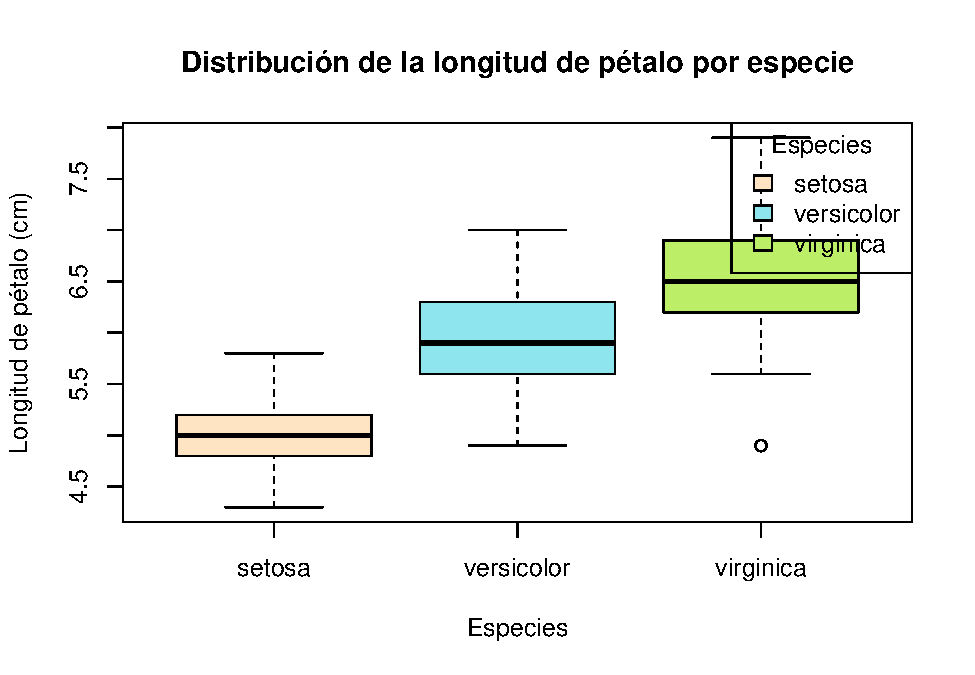
\includegraphics[keepaspectratio]{Tarea-Script_files/figure-latex/unnamed-chunk-1-1.pdf}}

\begin{Shaded}
\begin{Highlighting}[]
\CommentTok{\# k(k{-}1)/2 pares de medias \textgreater{} 5(5{-}1)/2 = 5(4)/2 = 10 posibles pares de medias.}


\CommentTok{\# Posibles pares de medias {-}{-}{-}{-}{-}{-}{-}{-}{-}{-}{-}{-}{-}{-}{-}{-}{-}{-}{-}{-}{-}{-}{-}{-}{-}{-}{-}{-}{-}{-}{-}{-}{-}{-}{-}{-}{-}{-}{-}{-}{-}{-}{-}{-}{-}{-}{-}{-}}

\CommentTok{\#**Posibilidad 1**}
\CommentTok{\# H0 = μ(Grayson’s Pond) = μ(Beaver Lake)}
\CommentTok{\# H1 = μ(Grayson’s Pond) ≠ μ(Beaver Lake)}

\CommentTok{\#**Posibilidad 2**}
\CommentTok{\# H0 = μ(Grayson’s Pond) = μ(Angler’s Cove)}
\CommentTok{\# H1 = μ(Grayson’s Pond) ≠ μ(Angler’s Cove)}

\CommentTok{\#**Posibilidad 3**}
\CommentTok{\# H0 = μ(Grayson’s Pond) = μ(Appletree Lake)}
\CommentTok{\# H1 = μ(Grayson’s Pond) ≠ μ(Appletree Lake)}

\CommentTok{\#**Posibilidad 4**}
\CommentTok{\# H0 = μ(Grayson’s Pond) = μ(Rock River)}
\CommentTok{\# H1 = μ(Grayson’s Pond) ≠ μ(Rock River)}

\CommentTok{\#**Posibilidad 5**}
\CommentTok{\# H0 = μ(Beaver Lake) = μ(Angler’s Cove)}
\CommentTok{\# H1 = μ(Beaver Lake) ≠ μ(Angler’s Cove)}

\CommentTok{\#**Posibilidad 6**}
\CommentTok{\# H0 = μ(Beaver Lake) = μ(Appletree Lake)}
\CommentTok{\# H1 = μ(Beaver Lake) ≠ μ(Appletree Lake)}

\CommentTok{\#**Posibilidad 7**}
\CommentTok{\# H0 = μ(Beaver Lake) = μ(Rock River)}
\CommentTok{\# H1 = μ(Beaver Lake) ≠ μ(Rock River)}

\CommentTok{\#**Posibilidad 8**}
\CommentTok{\# H0 = μ(Angler’s Cove) = μ(Appletree Lake)}
\CommentTok{\# H1 = μ(Angler’s Cove) ≠ μ(Appletree Lake)}

\CommentTok{\#**Posibilidad 9**}
\CommentTok{\# H0 = μ(Angler’s Cove) = μ(Rock River)}
\CommentTok{\# H1 = μ(Angler’s Cove) ≠ μ(Rock River)}

\CommentTok{\#**Posibilidad 10**}
\CommentTok{\# H0 = μ(Appletree Lake) = μ(Rock River)}
\CommentTok{\# H1 = μ(Appletree Lake) ≠ μ(Rock River)}

\FunctionTok{qt}\NormalTok{(}\FloatTok{0.975}\NormalTok{, }\DecValTok{25}\NormalTok{) }\CommentTok{\# 0.975 \%confianza, 25(30 resultados{-}5 factores)}
\end{Highlighting}
\end{Shaded}

\begin{verbatim}
## [1] 2.059539
\end{verbatim}

\begin{Shaded}
\begin{Highlighting}[]
\CommentTok{\# 2.059539}

\FunctionTok{sqrt}\NormalTok{((}\DecValTok{2}\SpecialCharTok{*}\FloatTok{9.8}\NormalTok{)}\SpecialCharTok{/}\DecValTok{6}\NormalTok{)}\SpecialCharTok{*}\FunctionTok{qt}\NormalTok{(}\FloatTok{0.975}\NormalTok{, }\DecValTok{25}\NormalTok{) }\CommentTok{\# 2(qt),9.8(mean sq)/6(muestras)}
\end{Highlighting}
\end{Shaded}

\begin{verbatim}
## [1] 3.722394
\end{verbatim}

\begin{Shaded}
\begin{Highlighting}[]
\CommentTok{\#**3.722394** valor mínimo entre medias}
\CommentTok{\# 3.72 mg/ml}

\FunctionTok{tapply}\NormalTok{(estroncio\_long}\SpecialCharTok{$}\NormalTok{Concentracion, estroncio\_long}\SpecialCharTok{$}\NormalTok{Cuerpo\_agua, mean)}
\end{Highlighting}
\end{Shaded}

\begin{verbatim}
##  Angler.s.Cove Appletree.Lake    Beaver.Lake Grayson.s.Pond     Rock.River 
##       44.08333       41.10000       40.23333       32.08333       58.30000
\end{verbatim}

\begin{Shaded}
\begin{Highlighting}[]
\FunctionTok{library}\NormalTok{(dplyr)}
\FunctionTok{library}\NormalTok{(knitr)}

\NormalTok{medias }\OtherTok{\textless{}{-}} \FunctionTok{tapply}\NormalTok{(estroncio\_long}\SpecialCharTok{$}\NormalTok{Concentracion, estroncio\_long}\SpecialCharTok{$}\NormalTok{Cuerpo\_agua, mean)}
\FunctionTok{kable}\NormalTok{(medias, }\AttributeTok{caption =} \StringTok{"Medias de concentración de estroncio (mg/ml) por cuerpo de agua"}\NormalTok{,}
      \AttributeTok{col.names =} \FunctionTok{c}\NormalTok{(}\StringTok{"Cuerpo de agua"}\NormalTok{, }\StringTok{"Media (mg/ml)"}\NormalTok{))}
\end{Highlighting}
\end{Shaded}

\begin{longtable}[]{@{}lr@{}}
\caption{Medias de concentración de estroncio (mg/ml) por cuerpo de
agua}\tabularnewline
\toprule\noalign{}
Cuerpo de agua & Media (mg/ml) \\
\midrule\noalign{}
\endfirsthead
\toprule\noalign{}
Cuerpo de agua & Media (mg/ml) \\
\midrule\noalign{}
\endhead
\bottomrule\noalign{}
\endlastfoot
Angler.s.Cove & 44.08333 \\
Appletree.Lake & 41.10000 \\
Beaver.Lake & 40.23333 \\
Grayson.s.Pond & 32.08333 \\
Rock.River & 58.30000 \\
\end{longtable}

\begin{Shaded}
\begin{Highlighting}[]
\NormalTok{LSD }\OtherTok{\textless{}{-}} \FloatTok{3.72}

\CommentTok{\# Diferencia entre medias {-}{-}{-}{-}{-}{-}{-}{-}{-}{-}{-}{-}{-}{-}{-}{-}{-}{-}{-}{-}{-}{-}{-}{-}{-}{-}{-}{-}{-}{-}{-}{-}{-}{-}{-}{-}{-}{-}{-}{-}{-}{-}{-}{-}{-}{-}{-}{-}{-}}

\NormalTok{Posibilidad1 }\OtherTok{\textless{}{-}}\NormalTok{ medias[}\StringTok{"Grayson.s.Pond"}\NormalTok{] }\SpecialCharTok{{-}}\NormalTok{ medias[}\StringTok{"Beaver.Lake"}\NormalTok{]}
\NormalTok{Posibilidad1; }\FunctionTok{ifelse}\NormalTok{(}\FunctionTok{abs}\NormalTok{(Posibilidad1) }\SpecialCharTok{\textgreater{}}\NormalTok{ LSD, }\StringTok{"Significativa"}\NormalTok{, }\StringTok{"No significativa"}\NormalTok{)}
\end{Highlighting}
\end{Shaded}

\begin{verbatim}
## Grayson.s.Pond 
##          -8.15
\end{verbatim}

\begin{verbatim}
##  Grayson.s.Pond 
## "Significativa"
\end{verbatim}

\begin{Shaded}
\begin{Highlighting}[]
\CommentTok{\# {-}8.15 Significativa}

\NormalTok{Posibilidad2 }\OtherTok{\textless{}{-}}\NormalTok{ medias[}\StringTok{"Grayson.s.Pond"}\NormalTok{] }\SpecialCharTok{{-}}\NormalTok{ medias[}\StringTok{"Angler.s.Cove"}\NormalTok{]}
\NormalTok{Posibilidad2; }\FunctionTok{ifelse}\NormalTok{(}\FunctionTok{abs}\NormalTok{(Posibilidad2) }\SpecialCharTok{\textgreater{}}\NormalTok{ LSD, }\StringTok{"Significativa"}\NormalTok{, }\StringTok{"No significativa"}\NormalTok{)}
\end{Highlighting}
\end{Shaded}

\begin{verbatim}
## Grayson.s.Pond 
##            -12
\end{verbatim}

\begin{verbatim}
##  Grayson.s.Pond 
## "Significativa"
\end{verbatim}

\begin{Shaded}
\begin{Highlighting}[]
\CommentTok{\# {-}12.0 Significativa}

\NormalTok{Posibilidad3 }\OtherTok{\textless{}{-}}\NormalTok{ medias[}\StringTok{"Grayson.s.Pond"}\NormalTok{] }\SpecialCharTok{{-}}\NormalTok{ medias[}\StringTok{"Appletree.Lake"}\NormalTok{]}
\NormalTok{Posibilidad3; }\FunctionTok{ifelse}\NormalTok{(}\FunctionTok{abs}\NormalTok{(Posibilidad3) }\SpecialCharTok{\textgreater{}}\NormalTok{ LSD, }\StringTok{"Significativa"}\NormalTok{, }\StringTok{"No significativa"}\NormalTok{)}
\end{Highlighting}
\end{Shaded}

\begin{verbatim}
## Grayson.s.Pond 
##      -9.016667
\end{verbatim}

\begin{verbatim}
##  Grayson.s.Pond 
## "Significativa"
\end{verbatim}

\begin{Shaded}
\begin{Highlighting}[]
\CommentTok{\# {-}9.017 Significativa}

\NormalTok{Posibilidad4 }\OtherTok{\textless{}{-}}\NormalTok{ medias[}\StringTok{"Grayson.s.Pond"}\NormalTok{] }\SpecialCharTok{{-}}\NormalTok{ medias[}\StringTok{"Rock.River"}\NormalTok{]}
\NormalTok{Posibilidad4; }\FunctionTok{ifelse}\NormalTok{(}\FunctionTok{abs}\NormalTok{(Posibilidad4) }\SpecialCharTok{\textgreater{}}\NormalTok{ LSD, }\StringTok{"Significativa"}\NormalTok{, }\StringTok{"No significativa"}\NormalTok{)}
\end{Highlighting}
\end{Shaded}

\begin{verbatim}
## Grayson.s.Pond 
##      -26.21667
\end{verbatim}

\begin{verbatim}
##  Grayson.s.Pond 
## "Significativa"
\end{verbatim}

\begin{Shaded}
\begin{Highlighting}[]
\CommentTok{\# {-}26.217 Significativa}

\NormalTok{Posibilidad5 }\OtherTok{\textless{}{-}}\NormalTok{ medias[}\StringTok{"Beaver.Lake"}\NormalTok{] }\SpecialCharTok{{-}}\NormalTok{ medias[}\StringTok{"Angler.s.Cove"}\NormalTok{]}
\NormalTok{Posibilidad5; }\FunctionTok{ifelse}\NormalTok{(}\FunctionTok{abs}\NormalTok{(Posibilidad5) }\SpecialCharTok{\textgreater{}}\NormalTok{ LSD, }\StringTok{"Significativa"}\NormalTok{, }\StringTok{"No significativa"}\NormalTok{)}
\end{Highlighting}
\end{Shaded}

\begin{verbatim}
## Beaver.Lake 
##       -3.85
\end{verbatim}

\begin{verbatim}
##     Beaver.Lake 
## "Significativa"
\end{verbatim}

\begin{Shaded}
\begin{Highlighting}[]
\CommentTok{\# {-}3.85 Significativa}

\NormalTok{Posibilidad6 }\OtherTok{\textless{}{-}}\NormalTok{ medias[}\StringTok{"Beaver.Lake"}\NormalTok{] }\SpecialCharTok{{-}}\NormalTok{ medias[}\StringTok{"Appletree.Lake"}\NormalTok{]}
\NormalTok{Posibilidad6; }\FunctionTok{ifelse}\NormalTok{(}\FunctionTok{abs}\NormalTok{(Posibilidad6) }\SpecialCharTok{\textgreater{}}\NormalTok{ LSD, }\StringTok{"Significativa"}\NormalTok{, }\StringTok{"No significativa"}\NormalTok{)}
\end{Highlighting}
\end{Shaded}

\begin{verbatim}
## Beaver.Lake 
##  -0.8666667
\end{verbatim}

\begin{verbatim}
##        Beaver.Lake 
## "No significativa"
\end{verbatim}

\begin{Shaded}
\begin{Highlighting}[]
\CommentTok{\# {-}0.867 No significativa}

\NormalTok{Posibilidad7 }\OtherTok{\textless{}{-}}\NormalTok{ medias[}\StringTok{"Beaver.Lake"}\NormalTok{] }\SpecialCharTok{{-}}\NormalTok{ medias[}\StringTok{"Rock.River"}\NormalTok{]}
\NormalTok{Posibilidad7; }\FunctionTok{ifelse}\NormalTok{(}\FunctionTok{abs}\NormalTok{(Posibilidad7) }\SpecialCharTok{\textgreater{}}\NormalTok{ LSD, }\StringTok{"Significativa"}\NormalTok{, }\StringTok{"No significativa"}\NormalTok{)}
\end{Highlighting}
\end{Shaded}

\begin{verbatim}
## Beaver.Lake 
##   -18.06667
\end{verbatim}

\begin{verbatim}
##     Beaver.Lake 
## "Significativa"
\end{verbatim}

\begin{Shaded}
\begin{Highlighting}[]
\CommentTok{\# {-}18.067 Significativa}

\NormalTok{Posibilidad8 }\OtherTok{\textless{}{-}}\NormalTok{ medias[}\StringTok{"Angler.s.Cove"}\NormalTok{] }\SpecialCharTok{{-}}\NormalTok{ medias[}\StringTok{"Appletree.Lake"}\NormalTok{]}
\NormalTok{Posibilidad8; }\FunctionTok{ifelse}\NormalTok{(}\FunctionTok{abs}\NormalTok{(Posibilidad8) }\SpecialCharTok{\textgreater{}}\NormalTok{ LSD, }\StringTok{"Significativa"}\NormalTok{, }\StringTok{"No significativa"}\NormalTok{)}
\end{Highlighting}
\end{Shaded}

\begin{verbatim}
## Angler.s.Cove 
##      2.983333
\end{verbatim}

\begin{verbatim}
##      Angler.s.Cove 
## "No significativa"
\end{verbatim}

\begin{Shaded}
\begin{Highlighting}[]
\CommentTok{\# 2.983 No significativa}

\NormalTok{Posibilidad9 }\OtherTok{\textless{}{-}}\NormalTok{ medias[}\StringTok{"Angler.s.Cove"}\NormalTok{] }\SpecialCharTok{{-}}\NormalTok{ medias[}\StringTok{"Rock.River"}\NormalTok{]}
\NormalTok{Posibilidad9; }\FunctionTok{ifelse}\NormalTok{(}\FunctionTok{abs}\NormalTok{(Posibilidad9) }\SpecialCharTok{\textgreater{}}\NormalTok{ LSD, }\StringTok{"Significativa"}\NormalTok{, }\StringTok{"No significativa"}\NormalTok{)}
\end{Highlighting}
\end{Shaded}

\begin{verbatim}
## Angler.s.Cove 
##     -14.21667
\end{verbatim}

\begin{verbatim}
##   Angler.s.Cove 
## "Significativa"
\end{verbatim}

\begin{Shaded}
\begin{Highlighting}[]
\CommentTok{\# {-}14.217 Significativa}

\NormalTok{Posibilidad10 }\OtherTok{\textless{}{-}}\NormalTok{ medias[}\StringTok{"Appletree.Lake"}\NormalTok{] }\SpecialCharTok{{-}}\NormalTok{ medias[}\StringTok{"Rock.River"}\NormalTok{]}
\NormalTok{Posibilidad10; }\FunctionTok{ifelse}\NormalTok{(}\FunctionTok{abs}\NormalTok{(Posibilidad10) }\SpecialCharTok{\textgreater{}}\NormalTok{ LSD, }\StringTok{"Significativa"}\NormalTok{, }\StringTok{"No significativa"}\NormalTok{)}
\end{Highlighting}
\end{Shaded}

\begin{verbatim}
## Appletree.Lake 
##          -17.2
\end{verbatim}

\begin{verbatim}
##  Appletree.Lake 
## "Significativa"
\end{verbatim}

\begin{Shaded}
\begin{Highlighting}[]
\CommentTok{\# {-}17.2 Significativa}

\FunctionTok{library}\NormalTok{(knitr)}

\NormalTok{resultados }\OtherTok{\textless{}{-}} \FunctionTok{data.frame}\NormalTok{(}
  \AttributeTok{Comparacion =} \FunctionTok{c}\NormalTok{(}
    \StringTok{"Grayson’s Pond vs Beaver Lake"}\NormalTok{,}
    \StringTok{"Grayson’s Pond vs Angler’s Cove"}\NormalTok{,}
    \StringTok{"Grayson’s Pond vs Appletree Lake"}\NormalTok{,}
    \StringTok{"Grayson’s Pond vs Rock River"}\NormalTok{,}
    \StringTok{"Beaver Lake vs Angler’s Cove"}\NormalTok{,}
    \StringTok{"Beaver Lake vs Appletree Lake"}\NormalTok{,}
    \StringTok{"Beaver Lake vs Rock River"}\NormalTok{,}
    \StringTok{"Angler’s Cove vs Appletree Lake"}\NormalTok{,}
    \StringTok{"Angler’s Cove vs Rock River"}\NormalTok{,}
    \StringTok{"Appletree Lake vs Rock River"}
\NormalTok{  ),}
  \AttributeTok{Diferencia =} \FunctionTok{c}\NormalTok{(}\SpecialCharTok{{-}}\FloatTok{8.15}\NormalTok{, }\SpecialCharTok{{-}}\FloatTok{12.00}\NormalTok{, }\SpecialCharTok{{-}}\FloatTok{9.017}\NormalTok{, }\SpecialCharTok{{-}}\FloatTok{26.217}\NormalTok{, }\SpecialCharTok{{-}}\FloatTok{3.85}\NormalTok{, }\SpecialCharTok{{-}}\FloatTok{0.867}\NormalTok{, }\SpecialCharTok{{-}}\FloatTok{18.067}\NormalTok{, }\FloatTok{2.983}\NormalTok{, }\SpecialCharTok{{-}}\FloatTok{14.217}\NormalTok{, }\SpecialCharTok{{-}}\FloatTok{17.2}\NormalTok{),}
  \AttributeTok{Significancia =} \FunctionTok{c}\NormalTok{(}\StringTok{"Significativa"}\NormalTok{, }\StringTok{"Significativa"}\NormalTok{, }\StringTok{"Significativa"}\NormalTok{, }\StringTok{"Significativa"}\NormalTok{,}
                    \StringTok{"Significativa"}\NormalTok{, }\StringTok{"No significativa"}\NormalTok{, }\StringTok{"Significativa"}\NormalTok{,}
                    \StringTok{"No significativa"}\NormalTok{, }\StringTok{"Significativa"}\NormalTok{, }\StringTok{"Significativa"}\NormalTok{)}
\NormalTok{)}

\FunctionTok{kable}\NormalTok{(resultados, }\AttributeTok{caption =} \StringTok{"Resultados LSD de comparación entre pares de medias"}\NormalTok{,}
      \AttributeTok{col.names =} \FunctionTok{c}\NormalTok{(}\StringTok{"Pares de medias"}\NormalTok{, }\StringTok{"Diferencia (mg/ml)"}\NormalTok{, }\StringTok{"Resultado LSD"}\NormalTok{))}
\end{Highlighting}
\end{Shaded}

\begin{longtable}[]{@{}
  >{\raggedright\arraybackslash}p{(\linewidth - 4\tabcolsep) * \real{0.4783}}
  >{\raggedleft\arraybackslash}p{(\linewidth - 4\tabcolsep) * \real{0.2754}}
  >{\raggedright\arraybackslash}p{(\linewidth - 4\tabcolsep) * \real{0.2464}}@{}}
\caption{Resultados LSD de comparación entre pares de
medias}\tabularnewline
\toprule\noalign{}
\begin{minipage}[b]{\linewidth}\raggedright
Pares de medias
\end{minipage} & \begin{minipage}[b]{\linewidth}\raggedleft
Diferencia (mg/ml)
\end{minipage} & \begin{minipage}[b]{\linewidth}\raggedright
Resultado LSD
\end{minipage} \\
\midrule\noalign{}
\endfirsthead
\toprule\noalign{}
\begin{minipage}[b]{\linewidth}\raggedright
Pares de medias
\end{minipage} & \begin{minipage}[b]{\linewidth}\raggedleft
Diferencia (mg/ml)
\end{minipage} & \begin{minipage}[b]{\linewidth}\raggedright
Resultado LSD
\end{minipage} \\
\midrule\noalign{}
\endhead
\bottomrule\noalign{}
\endlastfoot
Grayson's Pond vs Beaver Lake & -8.150 & Significativa \\
Grayson's Pond vs Angler's Cove & -12.000 & Significativa \\
Grayson's Pond vs Appletree Lake & -9.017 & Significativa \\
Grayson's Pond vs Rock River & -26.217 & Significativa \\
Beaver Lake vs Angler's Cove & -3.850 & Significativa \\
Beaver Lake vs Appletree Lake & -0.867 & No significativa \\
Beaver Lake vs Rock River & -18.067 & Significativa \\
Angler's Cove vs Appletree Lake & 2.983 & No significativa \\
Angler's Cove vs Rock River & -14.217 & Significativa \\
Appletree Lake vs Rock River & -17.200 & Significativa \\
\end{longtable}

\begin{Shaded}
\begin{Highlighting}[]
\CommentTok{\# Tukey HSD {-}{-}{-}{-}{-}{-}{-}{-}{-}{-}{-}{-}{-}{-}{-}{-}{-}{-}{-}{-}{-}{-}{-}{-}{-}{-}{-}{-}{-}{-}{-}{-}{-}{-}{-}{-}{-}{-}{-}{-}{-}{-}{-}{-}{-}{-}{-}{-}{-}{-}{-}{-}{-}{-}{-}{-}{-}{-}{-}{-}{-}{-}{-}}

\FunctionTok{sqrt}\NormalTok{(}\FloatTok{9.8}\SpecialCharTok{/}\DecValTok{6}\NormalTok{) }\SpecialCharTok{*} \FunctionTok{qtukey}\NormalTok{(}\FloatTok{0.95}\NormalTok{, }\AttributeTok{nmeans =} \DecValTok{5}\NormalTok{, }\AttributeTok{df =} \DecValTok{25}\NormalTok{)}
\end{Highlighting}
\end{Shaded}

\begin{verbatim}
## [1] 5.308078
\end{verbatim}

\begin{Shaded}
\begin{Highlighting}[]
\CommentTok{\# 5.308078}

\FunctionTok{TukeyHSD}\NormalTok{(estroncio\_long.aov)}
\end{Highlighting}
\end{Shaded}

\begin{verbatim}
##   Tukey multiple comparisons of means
##     95% family-wise confidence level
## 
## Fit: aov(formula = estroncio_long$Concentracion ~ estroncio_long$Cuerpo_agua)
## 
## $`estroncio_long$Cuerpo_agua`
##                                      diff        lwr       upr     p adj
## Appletree.Lake-Angler.s.Cove   -2.9833333  -8.281979  2.315312 0.4791100
## Beaver.Lake-Angler.s.Cove      -3.8500000  -9.148645  1.448645 0.2376217
## Grayson.s.Pond-Angler.s.Cove  -12.0000000 -17.298645 -6.701355 0.0000053
## Rock.River-Angler.s.Cove       14.2166667   8.918021 19.515312 0.0000003
## Beaver.Lake-Appletree.Lake     -0.8666667  -6.165312  4.431979 0.9884803
## Grayson.s.Pond-Appletree.Lake  -9.0166667 -14.315312 -3.718021 0.0003339
## Rock.River-Appletree.Lake      17.2000000  11.901355 22.498645 0.0000000
## Grayson.s.Pond-Beaver.Lake     -8.1500000 -13.448645 -2.851355 0.0011293
## Rock.River-Beaver.Lake         18.0666667  12.768021 23.365312 0.0000000
## Rock.River-Grayson.s.Pond      26.2166667  20.918021 31.515312 0.0000000
\end{verbatim}

\begin{Shaded}
\begin{Highlighting}[]
\FunctionTok{plot}\NormalTok{(}\FunctionTok{TukeyHSD}\NormalTok{(estroncio\_long.aov), }\AttributeTok{las =} \DecValTok{1}\NormalTok{, }\AttributeTok{cex.axis =} \FloatTok{0.6}\NormalTok{)}
\end{Highlighting}
\end{Shaded}

\pandocbounded{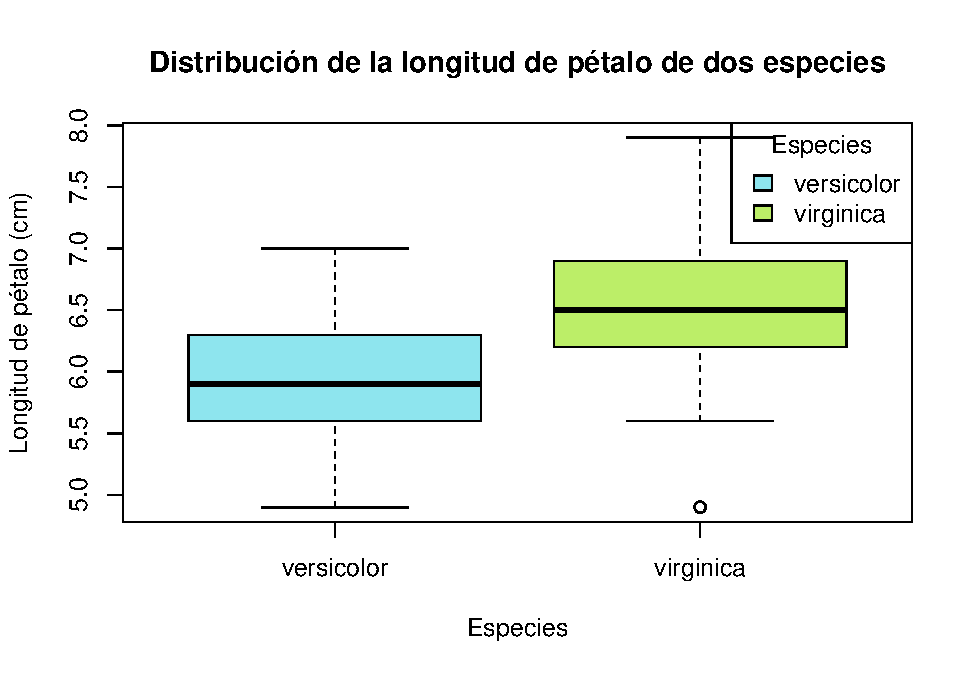
\includegraphics[keepaspectratio]{Tarea-Script_files/figure-latex/unnamed-chunk-1-2.pdf}}

\begin{Shaded}
\begin{Highlighting}[]
\NormalTok{PTukey }\OtherTok{\textless{}{-}} \FloatTok{5.31}

\NormalTok{Posibilidad1HSD }\OtherTok{\textless{}{-}}\NormalTok{ medias[}\StringTok{"Grayson.s.Pond"}\NormalTok{] }\SpecialCharTok{{-}}\NormalTok{ medias[}\StringTok{"Beaver.Lake"}\NormalTok{]}
\NormalTok{Posibilidad1HSD; }\FunctionTok{ifelse}\NormalTok{(}\FunctionTok{abs}\NormalTok{(Posibilidad1HSD) }\SpecialCharTok{\textgreater{}}\NormalTok{ PTukey, }\StringTok{"Significativa"}\NormalTok{, }\StringTok{"No significativa"}\NormalTok{)}
\end{Highlighting}
\end{Shaded}

\begin{verbatim}
## Grayson.s.Pond 
##          -8.15
\end{verbatim}

\begin{verbatim}
##  Grayson.s.Pond 
## "Significativa"
\end{verbatim}

\begin{Shaded}
\begin{Highlighting}[]
\CommentTok{\# {-}8.15 Significativa}

\NormalTok{Posibilidad2HSD }\OtherTok{\textless{}{-}}\NormalTok{ medias[}\StringTok{"Grayson.s.Pond"}\NormalTok{] }\SpecialCharTok{{-}}\NormalTok{ medias[}\StringTok{"Angler.s.Cove"}\NormalTok{]}
\NormalTok{Posibilidad2HSD; }\FunctionTok{ifelse}\NormalTok{(}\FunctionTok{abs}\NormalTok{(Posibilidad2HSD) }\SpecialCharTok{\textgreater{}}\NormalTok{ PTukey, }\StringTok{"Significativa"}\NormalTok{, }\StringTok{"No significativa"}\NormalTok{)}
\end{Highlighting}
\end{Shaded}

\begin{verbatim}
## Grayson.s.Pond 
##            -12
\end{verbatim}

\begin{verbatim}
##  Grayson.s.Pond 
## "Significativa"
\end{verbatim}

\begin{Shaded}
\begin{Highlighting}[]
\CommentTok{\# {-}12.0 Significativa}

\NormalTok{Posibilidad3HSD }\OtherTok{\textless{}{-}}\NormalTok{ medias[}\StringTok{"Grayson.s.Pond"}\NormalTok{] }\SpecialCharTok{{-}}\NormalTok{ medias[}\StringTok{"Appletree.Lake"}\NormalTok{]}
\NormalTok{Posibilidad3HSD; }\FunctionTok{ifelse}\NormalTok{(}\FunctionTok{abs}\NormalTok{(Posibilidad3HSD) }\SpecialCharTok{\textgreater{}}\NormalTok{ PTukey, }\StringTok{"Significativa"}\NormalTok{, }\StringTok{"No significativa"}\NormalTok{)}
\end{Highlighting}
\end{Shaded}

\begin{verbatim}
## Grayson.s.Pond 
##      -9.016667
\end{verbatim}

\begin{verbatim}
##  Grayson.s.Pond 
## "Significativa"
\end{verbatim}

\begin{Shaded}
\begin{Highlighting}[]
\CommentTok{\# {-}9.017 Significativa}

\NormalTok{Posibilidad4HSD }\OtherTok{\textless{}{-}}\NormalTok{ medias[}\StringTok{"Grayson.s.Pond"}\NormalTok{] }\SpecialCharTok{{-}}\NormalTok{ medias[}\StringTok{"Rock.River"}\NormalTok{]}
\NormalTok{Posibilidad4HSD; }\FunctionTok{ifelse}\NormalTok{(}\FunctionTok{abs}\NormalTok{(Posibilidad4HSD) }\SpecialCharTok{\textgreater{}}\NormalTok{ PTukey, }\StringTok{"Significativa"}\NormalTok{, }\StringTok{"No significativa"}\NormalTok{)}
\end{Highlighting}
\end{Shaded}

\begin{verbatim}
## Grayson.s.Pond 
##      -26.21667
\end{verbatim}

\begin{verbatim}
##  Grayson.s.Pond 
## "Significativa"
\end{verbatim}

\begin{Shaded}
\begin{Highlighting}[]
\CommentTok{\# {-}26.217 Significativa}

\NormalTok{Posibilidad5HSD }\OtherTok{\textless{}{-}}\NormalTok{ medias[}\StringTok{"Beaver.Lake"}\NormalTok{] }\SpecialCharTok{{-}}\NormalTok{ medias[}\StringTok{"Angler.s.Cove"}\NormalTok{]}
\NormalTok{Posibilidad5HSD; }\FunctionTok{ifelse}\NormalTok{(}\FunctionTok{abs}\NormalTok{(Posibilidad5HSD) }\SpecialCharTok{\textgreater{}}\NormalTok{ PTukey, }\StringTok{"Significativa"}\NormalTok{, }\StringTok{"No significativa"}\NormalTok{)}
\end{Highlighting}
\end{Shaded}

\begin{verbatim}
## Beaver.Lake 
##       -3.85
\end{verbatim}

\begin{verbatim}
##        Beaver.Lake 
## "No significativa"
\end{verbatim}

\begin{Shaded}
\begin{Highlighting}[]
\CommentTok{\# {-}3.85 No significativa}

\NormalTok{Posibilidad6HSD }\OtherTok{\textless{}{-}}\NormalTok{ medias[}\StringTok{"Beaver.Lake"}\NormalTok{] }\SpecialCharTok{{-}}\NormalTok{ medias[}\StringTok{"Appletree.Lake"}\NormalTok{]}
\NormalTok{Posibilidad6HSD; }\FunctionTok{ifelse}\NormalTok{(}\FunctionTok{abs}\NormalTok{(Posibilidad6HSD) }\SpecialCharTok{\textgreater{}}\NormalTok{ PTukey, }\StringTok{"Significativa"}\NormalTok{, }\StringTok{"No significativa"}\NormalTok{)}
\end{Highlighting}
\end{Shaded}

\begin{verbatim}
## Beaver.Lake 
##  -0.8666667
\end{verbatim}

\begin{verbatim}
##        Beaver.Lake 
## "No significativa"
\end{verbatim}

\begin{Shaded}
\begin{Highlighting}[]
\CommentTok{\# {-}0.867 No significativa}

\NormalTok{Posibilidad7HSD }\OtherTok{\textless{}{-}}\NormalTok{ medias[}\StringTok{"Beaver.Lake"}\NormalTok{] }\SpecialCharTok{{-}}\NormalTok{ medias[}\StringTok{"Rock.River"}\NormalTok{]}
\NormalTok{Posibilidad7HSD; }\FunctionTok{ifelse}\NormalTok{(}\FunctionTok{abs}\NormalTok{(Posibilidad7HSD) }\SpecialCharTok{\textgreater{}}\NormalTok{ PTukey, }\StringTok{"Significativa"}\NormalTok{, }\StringTok{"No significativa"}\NormalTok{)}
\end{Highlighting}
\end{Shaded}

\begin{verbatim}
## Beaver.Lake 
##   -18.06667
\end{verbatim}

\begin{verbatim}
##     Beaver.Lake 
## "Significativa"
\end{verbatim}

\begin{Shaded}
\begin{Highlighting}[]
\CommentTok{\# {-}18.067 Significativa}

\NormalTok{Posibilidad8HSD }\OtherTok{\textless{}{-}}\NormalTok{ medias[}\StringTok{"Angler.s.Cove"}\NormalTok{] }\SpecialCharTok{{-}}\NormalTok{ medias[}\StringTok{"Appletree.Lake"}\NormalTok{]}
\NormalTok{Posibilidad8HSD; }\FunctionTok{ifelse}\NormalTok{(}\FunctionTok{abs}\NormalTok{(Posibilidad8HSD) }\SpecialCharTok{\textgreater{}}\NormalTok{ PTukey, }\StringTok{"Significativa"}\NormalTok{, }\StringTok{"No significativa"}\NormalTok{)}
\end{Highlighting}
\end{Shaded}

\begin{verbatim}
## Angler.s.Cove 
##      2.983333
\end{verbatim}

\begin{verbatim}
##      Angler.s.Cove 
## "No significativa"
\end{verbatim}

\begin{Shaded}
\begin{Highlighting}[]
\CommentTok{\# 2.983 No significativa}

\NormalTok{Posibilidad9HSD }\OtherTok{\textless{}{-}}\NormalTok{ medias[}\StringTok{"Angler.s.Cove"}\NormalTok{] }\SpecialCharTok{{-}}\NormalTok{ medias[}\StringTok{"Rock.River"}\NormalTok{]}
\NormalTok{Posibilidad9HSD; }\FunctionTok{ifelse}\NormalTok{(}\FunctionTok{abs}\NormalTok{(Posibilidad9HSD) }\SpecialCharTok{\textgreater{}}\NormalTok{ PTukey, }\StringTok{"Significativa"}\NormalTok{, }\StringTok{"No significativa"}\NormalTok{)}
\end{Highlighting}
\end{Shaded}

\begin{verbatim}
## Angler.s.Cove 
##     -14.21667
\end{verbatim}

\begin{verbatim}
##   Angler.s.Cove 
## "Significativa"
\end{verbatim}

\begin{Shaded}
\begin{Highlighting}[]
\CommentTok{\# {-}14.217 Significativa}

\NormalTok{Posibilidad10HSD }\OtherTok{\textless{}{-}}\NormalTok{ medias[}\StringTok{"Appletree.Lake"}\NormalTok{] }\SpecialCharTok{{-}}\NormalTok{ medias[}\StringTok{"Rock.River"}\NormalTok{]}
\NormalTok{Posibilidad10HSD; }\FunctionTok{ifelse}\NormalTok{(}\FunctionTok{abs}\NormalTok{(Posibilidad10HSD) }\SpecialCharTok{\textgreater{}}\NormalTok{ PTukey, }\StringTok{"Significativa"}\NormalTok{, }\StringTok{"No significativa"}\NormalTok{)}
\end{Highlighting}
\end{Shaded}

\begin{verbatim}
## Appletree.Lake 
##          -17.2
\end{verbatim}

\begin{verbatim}
##  Appletree.Lake 
## "Significativa"
\end{verbatim}

\begin{Shaded}
\begin{Highlighting}[]
\CommentTok{\# {-}17.2 Significativa}

\FunctionTok{library}\NormalTok{(knitr)}

\NormalTok{resultadosHSD }\OtherTok{\textless{}{-}} \FunctionTok{data.frame}\NormalTok{(}
  \AttributeTok{Comparacion =} \FunctionTok{c}\NormalTok{(}
    \StringTok{"Grayson’s Pond vs Beaver Lake"}\NormalTok{,}
    \StringTok{"Grayson’s Pond vs Angler’s Cove"}\NormalTok{,}
    \StringTok{"Grayson’s Pond vs Appletree Lake"}\NormalTok{,}
    \StringTok{"Grayson’s Pond vs Rock River"}\NormalTok{,}
    \StringTok{"Beaver Lake vs Angler’s Cove"}\NormalTok{,}
    \StringTok{"Beaver Lake vs Appletree Lake"}\NormalTok{,}
    \StringTok{"Beaver Lake vs Rock River"}\NormalTok{,}
    \StringTok{"Angler’s Cove vs Appletree Lake"}\NormalTok{,}
    \StringTok{"Angler’s Cove vs Rock River"}\NormalTok{,}
    \StringTok{"Appletree Lake vs Rock River"}
\NormalTok{  ),}
  \AttributeTok{Diferencia =} \FunctionTok{c}\NormalTok{(}\SpecialCharTok{{-}}\FloatTok{8.15}\NormalTok{, }\SpecialCharTok{{-}}\FloatTok{12.00}\NormalTok{, }\SpecialCharTok{{-}}\FloatTok{9.017}\NormalTok{, }\SpecialCharTok{{-}}\FloatTok{26.217}\NormalTok{, }\SpecialCharTok{{-}}\FloatTok{3.85}\NormalTok{, }\SpecialCharTok{{-}}\FloatTok{0.867}\NormalTok{, }\SpecialCharTok{{-}}\FloatTok{18.067}\NormalTok{, }\FloatTok{2.983}\NormalTok{, }\SpecialCharTok{{-}}\FloatTok{14.217}\NormalTok{, }\SpecialCharTok{{-}}\FloatTok{17.2}\NormalTok{),}
  \AttributeTok{Significancia =} \FunctionTok{c}\NormalTok{(}\StringTok{"Significativa"}\NormalTok{, }\StringTok{"Significativa"}\NormalTok{, }\StringTok{"Significativa"}\NormalTok{, }\StringTok{"Significativa"}\NormalTok{,}
                    \StringTok{"No significativa"}\NormalTok{, }\StringTok{"No significativa"}\NormalTok{, }\StringTok{"Significativa"}\NormalTok{,}
                    \StringTok{"No significativa"}\NormalTok{, }\StringTok{"Significativa"}\NormalTok{, }\StringTok{"Significativa"}\NormalTok{)}
\NormalTok{)}

\FunctionTok{kable}\NormalTok{(resultadosHSD, }\AttributeTok{caption =} \StringTok{"Resultados Tukey HSD de comparación entre pares de medias"}\NormalTok{,}
      \AttributeTok{col.names =} \FunctionTok{c}\NormalTok{(}\StringTok{"Pares de medias"}\NormalTok{, }\StringTok{"Diferencia (mg/ml)"}\NormalTok{, }\StringTok{"Resultado Tukey HSD"}\NormalTok{))}
\end{Highlighting}
\end{Shaded}

\begin{longtable}[]{@{}
  >{\raggedright\arraybackslash}p{(\linewidth - 4\tabcolsep) * \real{0.4583}}
  >{\raggedleft\arraybackslash}p{(\linewidth - 4\tabcolsep) * \real{0.2639}}
  >{\raggedright\arraybackslash}p{(\linewidth - 4\tabcolsep) * \real{0.2778}}@{}}
\caption{Resultados Tukey HSD de comparación entre pares de
medias}\tabularnewline
\toprule\noalign{}
\begin{minipage}[b]{\linewidth}\raggedright
Pares de medias
\end{minipage} & \begin{minipage}[b]{\linewidth}\raggedleft
Diferencia (mg/ml)
\end{minipage} & \begin{minipage}[b]{\linewidth}\raggedright
Resultado Tukey HSD
\end{minipage} \\
\midrule\noalign{}
\endfirsthead
\toprule\noalign{}
\begin{minipage}[b]{\linewidth}\raggedright
Pares de medias
\end{minipage} & \begin{minipage}[b]{\linewidth}\raggedleft
Diferencia (mg/ml)
\end{minipage} & \begin{minipage}[b]{\linewidth}\raggedright
Resultado Tukey HSD
\end{minipage} \\
\midrule\noalign{}
\endhead
\bottomrule\noalign{}
\endlastfoot
Grayson's Pond vs Beaver Lake & -8.150 & Significativa \\
Grayson's Pond vs Angler's Cove & -12.000 & Significativa \\
Grayson's Pond vs Appletree Lake & -9.017 & Significativa \\
Grayson's Pond vs Rock River & -26.217 & Significativa \\
Beaver Lake vs Angler's Cove & -3.850 & No significativa \\
Beaver Lake vs Appletree Lake & -0.867 & No significativa \\
Beaver Lake vs Rock River & -18.067 & Significativa \\
Angler's Cove vs Appletree Lake & 2.983 & No significativa \\
Angler's Cove vs Rock River & -14.217 & Significativa \\
Appletree Lake vs Rock River & -17.200 & Significativa \\
\end{longtable}

\begin{Shaded}
\begin{Highlighting}[]
\CommentTok{\# Comparación entre LSD vs TukeyHSD {-}{-}{-}{-}{-}{-}{-}{-}{-}{-}{-}{-}{-}{-}{-}{-}{-}{-}{-}{-}{-}{-}{-}{-}{-}{-}{-}{-}{-}{-}{-}{-}{-}{-}{-}{-}{-}{-}{-}}

\FunctionTok{library}\NormalTok{(knitr)}

\NormalTok{comparaciones }\OtherTok{\textless{}{-}} \FunctionTok{c}\NormalTok{(}
  \StringTok{"Grayson’s Pond vs Beaver Lake"}\NormalTok{,}
  \StringTok{"Grayson’s Pond vs Angler’s Cove"}\NormalTok{,}
  \StringTok{"Grayson’s Pond vs Appletree Lake"}\NormalTok{,}
  \StringTok{"Grayson’s Pond vs Rock River"}\NormalTok{,}
  \StringTok{"Beaver Lake vs Angler’s Cove"}\NormalTok{,}
  \StringTok{"Beaver Lake vs Appletree Lake"}\NormalTok{,}
  \StringTok{"Beaver Lake vs Rock River"}\NormalTok{,}
  \StringTok{"Angler’s Cove vs Appletree Lake"}\NormalTok{,}
  \StringTok{"Angler’s Cove vs Rock River"}\NormalTok{,}
  \StringTok{"Appletree Lake vs Rock River"}
\NormalTok{)}

\NormalTok{diferencias }\OtherTok{\textless{}{-}} \FunctionTok{c}\NormalTok{(}\SpecialCharTok{{-}}\FloatTok{8.15}\NormalTok{, }\SpecialCharTok{{-}}\FloatTok{12.00}\NormalTok{, }\SpecialCharTok{{-}}\FloatTok{9.017}\NormalTok{, }\SpecialCharTok{{-}}\FloatTok{26.217}\NormalTok{, }\SpecialCharTok{{-}}\FloatTok{3.85}\NormalTok{, }\SpecialCharTok{{-}}\FloatTok{0.867}\NormalTok{, }\SpecialCharTok{{-}}\FloatTok{18.067}\NormalTok{, }\FloatTok{2.983}\NormalTok{, }\SpecialCharTok{{-}}\FloatTok{14.217}\NormalTok{, }\SpecialCharTok{{-}}\FloatTok{17.2}\NormalTok{)}

\NormalTok{resultado\_LSD }\OtherTok{\textless{}{-}} \FunctionTok{c}\NormalTok{(}\StringTok{"Significativa"}\NormalTok{, }\StringTok{"Significativa"}\NormalTok{, }\StringTok{"Significativa"}\NormalTok{, }\StringTok{"Significativa"}\NormalTok{,}
                   \StringTok{"Significativa"}\NormalTok{, }\StringTok{"No significativa"}\NormalTok{, }\StringTok{"Significativa"}\NormalTok{,}
                   \StringTok{"No significativa"}\NormalTok{, }\StringTok{"Significativa"}\NormalTok{, }\StringTok{"Significativa"}\NormalTok{)}

\NormalTok{resultado\_Tukey }\OtherTok{\textless{}{-}} \FunctionTok{c}\NormalTok{(}\StringTok{"Significativa"}\NormalTok{, }\StringTok{"Significativa"}\NormalTok{, }\StringTok{"Significativa"}\NormalTok{, }\StringTok{"Significativa"}\NormalTok{,}
                     \StringTok{"No significativa"}\NormalTok{, }\StringTok{"No significativa"}\NormalTok{, }\StringTok{"Significativa"}\NormalTok{,}
                     \StringTok{"No significativa"}\NormalTok{, }\StringTok{"Significativa"}\NormalTok{, }\StringTok{"Significativa"}\NormalTok{)}

\NormalTok{resultadosComparados }\OtherTok{\textless{}{-}} \FunctionTok{data.frame}\NormalTok{(}
  \StringTok{\textasciigrave{}}\AttributeTok{Pares de medias}\StringTok{\textasciigrave{}} \OtherTok{=}\NormalTok{ comparaciones,}
  \StringTok{\textasciigrave{}}\AttributeTok{Diferencia (mg/ml)}\StringTok{\textasciigrave{}} \OtherTok{=}\NormalTok{ diferencias,}
  \StringTok{\textasciigrave{}}\AttributeTok{Resultado LSD}\StringTok{\textasciigrave{}} \OtherTok{=}\NormalTok{ resultado\_LSD,}
  \StringTok{\textasciigrave{}}\AttributeTok{Resultado Tukey HSD}\StringTok{\textasciigrave{}} \OtherTok{=}\NormalTok{ resultado\_Tukey}
\NormalTok{)}


\FunctionTok{kable}\NormalTok{(resultadosComparados,}
      \AttributeTok{caption =} \StringTok{"Comparación de resultados LSD vs Tukey HSD entre pares de medias"}\NormalTok{,}
      \AttributeTok{col.names =} \FunctionTok{c}\NormalTok{(}\StringTok{"Pares de medias"}\NormalTok{, }\StringTok{"Diferencia (mg/ml)"}\NormalTok{, }\StringTok{"Resultado LSD"}\NormalTok{, }\StringTok{"Resultado Tukey HSD"}\NormalTok{))}
\end{Highlighting}
\end{Shaded}

\begin{longtable}[]{@{}
  >{\raggedright\arraybackslash}p{(\linewidth - 6\tabcolsep) * \real{0.3708}}
  >{\raggedleft\arraybackslash}p{(\linewidth - 6\tabcolsep) * \real{0.2135}}
  >{\raggedright\arraybackslash}p{(\linewidth - 6\tabcolsep) * \real{0.1910}}
  >{\raggedright\arraybackslash}p{(\linewidth - 6\tabcolsep) * \real{0.2247}}@{}}
\caption{Comparación de resultados LSD vs Tukey HSD entre pares de
medias}\tabularnewline
\toprule\noalign{}
\begin{minipage}[b]{\linewidth}\raggedright
Pares de medias
\end{minipage} & \begin{minipage}[b]{\linewidth}\raggedleft
Diferencia (mg/ml)
\end{minipage} & \begin{minipage}[b]{\linewidth}\raggedright
Resultado LSD
\end{minipage} & \begin{minipage}[b]{\linewidth}\raggedright
Resultado Tukey HSD
\end{minipage} \\
\midrule\noalign{}
\endfirsthead
\toprule\noalign{}
\begin{minipage}[b]{\linewidth}\raggedright
Pares de medias
\end{minipage} & \begin{minipage}[b]{\linewidth}\raggedleft
Diferencia (mg/ml)
\end{minipage} & \begin{minipage}[b]{\linewidth}\raggedright
Resultado LSD
\end{minipage} & \begin{minipage}[b]{\linewidth}\raggedright
Resultado Tukey HSD
\end{minipage} \\
\midrule\noalign{}
\endhead
\bottomrule\noalign{}
\endlastfoot
Grayson's Pond vs Beaver Lake & -8.150 & Significativa &
Significativa \\
Grayson's Pond vs Angler's Cove & -12.000 & Significativa &
Significativa \\
Grayson's Pond vs Appletree Lake & -9.017 & Significativa &
Significativa \\
Grayson's Pond vs Rock River & -26.217 & Significativa &
Significativa \\
Beaver Lake vs Angler's Cove & -3.850 & Significativa & No
significativa \\
Beaver Lake vs Appletree Lake & -0.867 & No significativa & No
significativa \\
Beaver Lake vs Rock River & -18.067 & Significativa & Significativa \\
Angler's Cove vs Appletree Lake & 2.983 & No significativa & No
significativa \\
Angler's Cove vs Rock River & -14.217 & Significativa & Significativa \\
Appletree Lake vs Rock River & -17.200 & Significativa &
Significativa \\
\end{longtable}

\begin{Shaded}
\begin{Highlighting}[]
\CommentTok{\# Interpretación {-}{-}{-}{-}{-}{-}{-}{-}{-}{-}{-}{-}{-}{-}{-}{-}{-}{-}{-}{-}{-}{-}{-}{-}{-}{-}{-}{-}{-}{-}{-}{-}{-}{-}{-}{-}{-}{-}{-}{-}{-}{-}{-}{-}{-}{-}{-}{-}{-}{-}{-}{-}{-}{-}{-}{-}{-}{-}}

\CommentTok{\# ¿Qué cuerpo de agua presenta las concentraciones más altas?}
\CommentTok{\# Grayson’s Pond y Beaver Lake.}

\CommentTok{\# ¿Qué sitios no difieren entre sí?}
\CommentTok{\# Según LSD: Beaver Lake vs Appletree Lake, Angler’s Cove vs Appletree Lake.}
\CommentTok{\# Según Tukey HSD: los mismos de LSD, más Beaver Lake vs Angler’s Cove.}

\CommentTok{\# ¿Qué implicaciones podrían tener estas diferencias en la calidad del agua?}
\CommentTok{\# Las diferencias en las concentraciones de estroncio entre cuerpos de agua }
\CommentTok{\# indican una variabilidad en la calidad. Los sitios con valores más altos podrían}
\CommentTok{\# estar expuestos a contaminación local o condiciones específicas, lo que}
\CommentTok{\# representa un riesgo potencial para la fauna y flora local. Asimismo, estas }
\CommentTok{\# diferencias pueden tener implicaciones en el uso humano del agua (consumo, }
\CommentTok{\# riego o recreación), por lo que los sitios con mayores concentraciones }
\CommentTok{\# requieren mayor monitoreo y gestión ambiental.}
\end{Highlighting}
\end{Shaded}


\end{document}
